% Created by tikzDevice version 0.6.1 on 2011-08-02 12:45:49
% !TEX encoding = UTF-8 Unicode
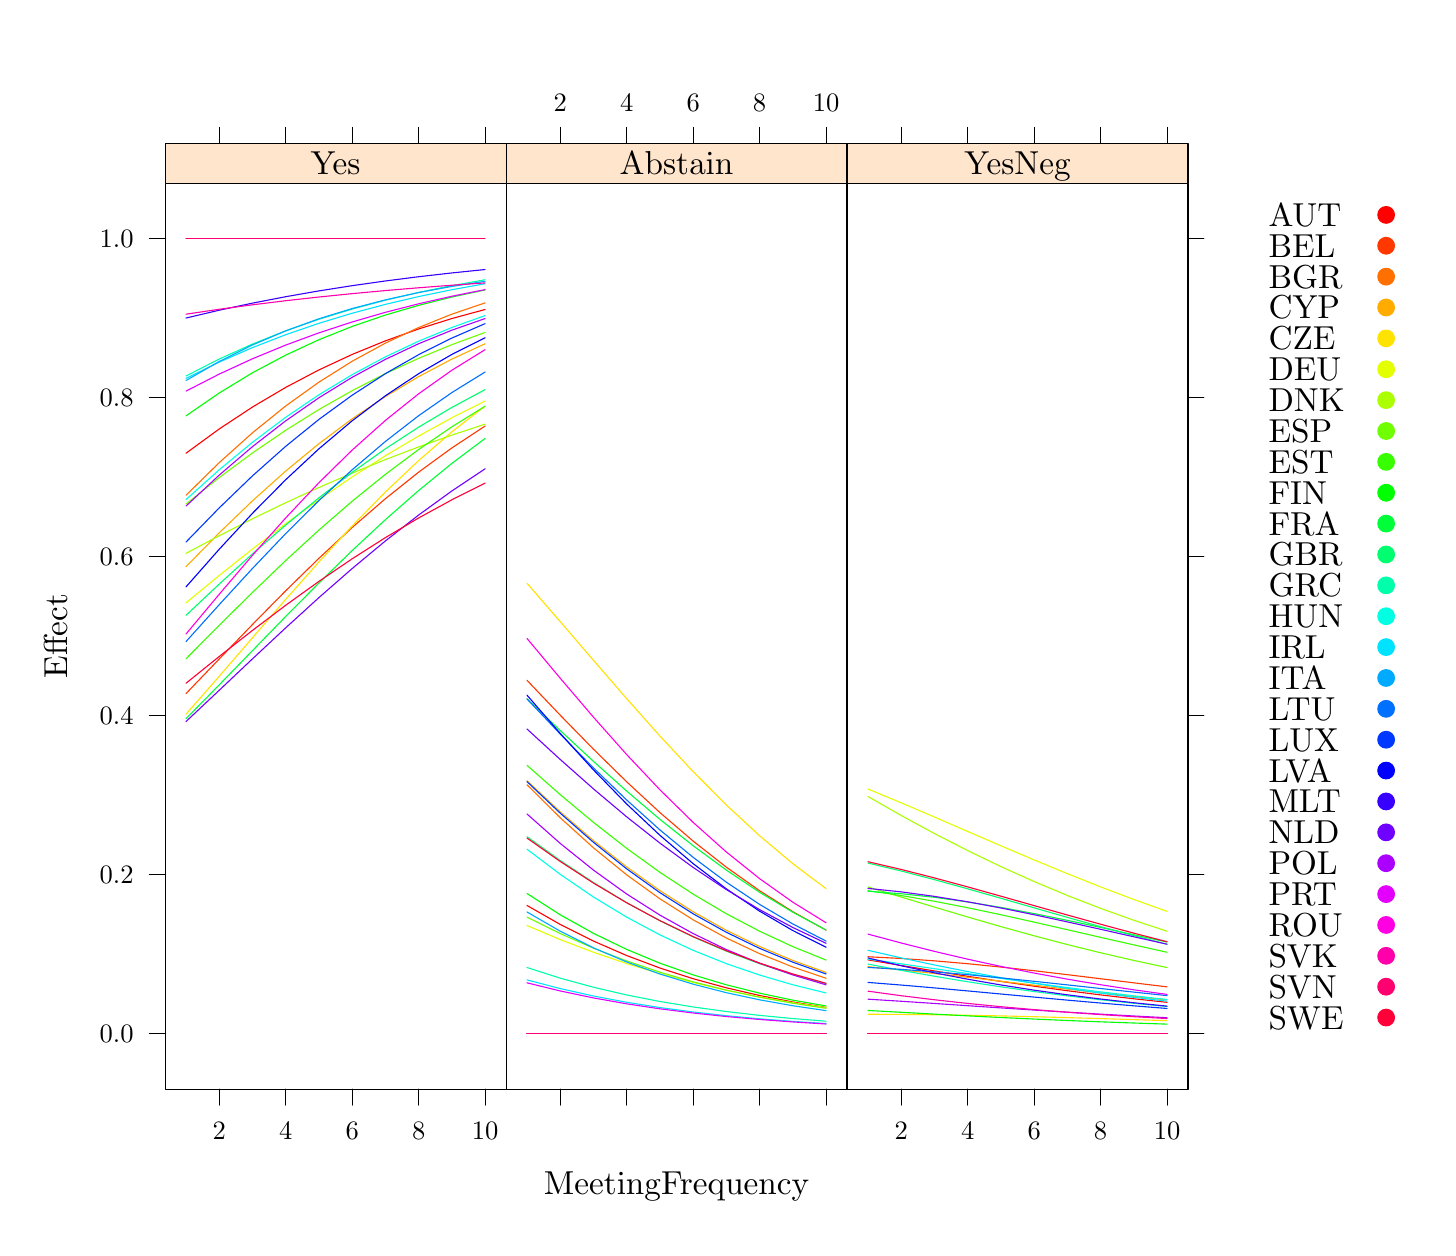
\begin{tikzpicture}[x=1pt,y=1pt]
\definecolor[named]{drawColor}{rgb}{0.00,0.00,0.00}
\definecolor[named]{fillColor}{rgb}{1.00,1.00,1.00}
\fill[color=fillColor,] (0,0) rectangle (505.89,433.62);
\begin{scope}
\path[clip] (  0.00,  0.00) rectangle (505.89,433.62);
\definecolor[named]{fillColor}{rgb}{0.00,0.00,0.00}
\end{scope}
\begin{scope}
\path[clip] (  0.00,  0.00) rectangle (505.89,433.62);
\definecolor[named]{fillColor}{rgb}{0.00,0.00,0.00}

\draw[fill opacity=0.00,draw opacity=0.00,] (  0.00,  0.00) rectangle (505.89,433.62);
\end{scope}
\begin{scope}
\path[clip] (  0.00,  0.00) rectangle (505.89,433.62);
\definecolor[named]{fillColor}{rgb}{0.00,0.00,0.00}
\end{scope}
\begin{scope}
\path[clip] (  0.00,  0.00) rectangle (505.89,433.62);
\definecolor[named]{fillColor}{rgb}{0.00,0.00,0.00}
\definecolor[named]{drawColor}{rgb}{0.00,0.00,0.00}

\node[color=drawColor,anchor=base,inner sep=0pt, outer sep=0pt, scale=  1.20] at (234.47, 12.04) {MeetingFrequency%
};
\end{scope}
\begin{scope}
\path[clip] (  0.00,  0.00) rectangle (505.89,433.62);
\definecolor[named]{fillColor}{rgb}{0.00,0.00,0.00}
\definecolor[named]{drawColor}{rgb}{0.00,0.00,0.00}

\node[rotate= 90.00,color=drawColor,anchor=base,inner sep=0pt, outer sep=0pt, scale=  1.20] at ( 14.29,213.72) {Effect%
};
\end{scope}
\begin{scope}
\path[clip] (  0.00,  0.00) rectangle (505.89,433.62);
\definecolor[named]{fillColor}{rgb}{0.00,0.00,0.00}
\end{scope}
\begin{scope}
\path[clip] (  0.00,  0.00) rectangle (505.89,433.62);
\definecolor[named]{fillColor}{rgb}{0.00,0.00,0.00}
\end{scope}
\begin{scope}
\path[clip] (  0.00,  0.00) rectangle (505.89,433.62);
\definecolor[named]{fillColor}{rgb}{0.00,0.00,0.00}
\end{scope}
\begin{scope}
\path[clip] ( 49.65, 50.02) rectangle (172.86,377.42);
\definecolor[named]{fillColor}{rgb}{0.00,0.00,0.00}
\end{scope}
\begin{scope}
\path[clip] (  0.00,  0.00) rectangle (505.89,433.62);
\definecolor[named]{fillColor}{rgb}{0.00,0.00,0.00}
\end{scope}
\begin{scope}
\path[clip] (  0.00,  0.00) rectangle (505.89,433.62);
\definecolor[named]{fillColor}{rgb}{0.00,0.00,0.00}
\definecolor[named]{drawColor}{rgb}{0.00,0.00,0.00}

\draw[color=drawColor,line cap=round,line join=round,fill opacity=0.00,] ( 69.22,391.87) -- ( 69.22,397.56);

\draw[color=drawColor,line cap=round,line join=round,fill opacity=0.00,] ( 93.24,391.87) -- ( 93.24,397.56);

\draw[color=drawColor,line cap=round,line join=round,fill opacity=0.00,] (117.26,391.87) -- (117.26,397.56);

\draw[color=drawColor,line cap=round,line join=round,fill opacity=0.00,] (141.28,391.87) -- (141.28,397.56);

\draw[color=drawColor,line cap=round,line join=round,fill opacity=0.00,] (165.29,391.87) -- (165.29,397.56);
\end{scope}
\begin{scope}
\path[clip] (  0.00,  0.00) rectangle (505.89,433.62);
\definecolor[named]{fillColor}{rgb}{0.00,0.00,0.00}
\end{scope}
\begin{scope}
\path[clip] (  0.00,  0.00) rectangle (505.89,433.62);
\definecolor[named]{fillColor}{rgb}{0.00,0.00,0.00}
\definecolor[named]{drawColor}{rgb}{0.00,0.00,0.00}

\draw[color=drawColor,line cap=round,line join=round,fill opacity=0.00,] ( 49.65, 70.12) -- ( 43.95, 70.12);

\draw[color=drawColor,line cap=round,line join=round,fill opacity=0.00,] ( 49.65,127.56) -- ( 43.95,127.56);

\draw[color=drawColor,line cap=round,line join=round,fill opacity=0.00,] ( 49.65,185.00) -- ( 43.95,185.00);

\draw[color=drawColor,line cap=round,line join=round,fill opacity=0.00,] ( 49.65,242.43) -- ( 43.95,242.43);

\draw[color=drawColor,line cap=round,line join=round,fill opacity=0.00,] ( 49.65,299.87) -- ( 43.95,299.87);

\draw[color=drawColor,line cap=round,line join=round,fill opacity=0.00,] ( 49.65,357.31) -- ( 43.95,357.31);

\node[color=drawColor,anchor=base east,inner sep=0pt, outer sep=0pt, scale=  0.96] at ( 38.26, 66.81) {0.0%
};

\node[color=drawColor,anchor=base east,inner sep=0pt, outer sep=0pt, scale=  0.96] at ( 38.26,124.25) {0.2%
};

\node[color=drawColor,anchor=base east,inner sep=0pt, outer sep=0pt, scale=  0.96] at ( 38.26,181.69) {0.4%
};

\node[color=drawColor,anchor=base east,inner sep=0pt, outer sep=0pt, scale=  0.96] at ( 38.26,239.13) {0.6%
};

\node[color=drawColor,anchor=base east,inner sep=0pt, outer sep=0pt, scale=  0.96] at ( 38.26,296.57) {0.8%
};

\node[color=drawColor,anchor=base east,inner sep=0pt, outer sep=0pt, scale=  0.96] at ( 38.26,354.01) {1.0%
};
\end{scope}
\begin{scope}
\path[clip] (  0.00,  0.00) rectangle (505.89,433.62);
\definecolor[named]{fillColor}{rgb}{0.00,0.00,0.00}
\end{scope}
\begin{scope}
\path[clip] (  0.00,  0.00) rectangle (505.89,433.62);
\definecolor[named]{fillColor}{rgb}{0.00,0.00,0.00}
\definecolor[named]{drawColor}{rgb}{0.00,0.00,0.00}

\draw[color=drawColor,line cap=round,line join=round,fill opacity=0.00,] ( 69.22, 50.02) -- ( 69.22, 44.32);

\draw[color=drawColor,line cap=round,line join=round,fill opacity=0.00,] ( 93.24, 50.02) -- ( 93.24, 44.32);

\draw[color=drawColor,line cap=round,line join=round,fill opacity=0.00,] (117.26, 50.02) -- (117.26, 44.32);

\draw[color=drawColor,line cap=round,line join=round,fill opacity=0.00,] (141.28, 50.02) -- (141.28, 44.32);

\draw[color=drawColor,line cap=round,line join=round,fill opacity=0.00,] (165.29, 50.02) -- (165.29, 44.32);

\node[color=drawColor,anchor=base,inner sep=0pt, outer sep=0pt, scale=  0.96] at ( 69.22, 32.02) {2%
};

\node[color=drawColor,anchor=base,inner sep=0pt, outer sep=0pt, scale=  0.96] at ( 93.24, 32.02) {4%
};

\node[color=drawColor,anchor=base,inner sep=0pt, outer sep=0pt, scale=  0.96] at (117.26, 32.02) {6%
};

\node[color=drawColor,anchor=base,inner sep=0pt, outer sep=0pt, scale=  0.96] at (141.28, 32.02) {8%
};

\node[color=drawColor,anchor=base,inner sep=0pt, outer sep=0pt, scale=  0.96] at (165.29, 32.02) {10%
};
\end{scope}
\begin{scope}
\path[clip] (  0.00,  0.00) rectangle (505.89,433.62);
\definecolor[named]{fillColor}{rgb}{0.00,0.00,0.00}
\end{scope}
\begin{scope}
\path[clip] ( 49.65, 50.02) rectangle (172.86,377.42);
\definecolor[named]{fillColor}{rgb}{0.00,0.00,0.00}
\definecolor[named]{drawColor}{rgb}{1.00,0.00,0.00}

\draw[color=drawColor,line cap=round,line join=round,fill opacity=0.00,] ( 57.21,279.84) --
	( 69.22,288.61) --
	( 81.23,296.53) --
	( 93.24,303.63) --
	(105.25,309.95) --
	(117.26,315.54) --
	(129.27,320.45) --
	(141.28,324.75) --
	(153.28,328.51) --
	(165.29,331.78);
\definecolor[named]{drawColor}{rgb}{1.00,0.22,0.00}

\draw[color=drawColor,line cap=round,line join=round,fill opacity=0.00,] ( 57.21,192.98) --
	( 69.22,205.49) --
	( 81.23,217.95) --
	( 93.24,230.14) --
	(105.25,241.88) --
	(117.26,253.01) --
	(129.27,263.41) --
	(141.28,273.01) --
	(153.28,281.76) --
	(165.29,289.67);
\definecolor[named]{drawColor}{rgb}{1.00,0.44,0.00}

\draw[color=drawColor,line cap=round,line join=round,fill opacity=0.00,] ( 57.21,264.63) --
	( 69.22,276.44) --
	( 81.23,287.22) --
	( 93.24,296.92) --
	(105.25,305.53) --
	(117.26,313.08) --
	(129.27,319.63) --
	(141.28,325.27) --
	(153.28,330.09) --
	(165.29,334.17);
\definecolor[named]{drawColor}{rgb}{1.00,0.67,0.00}

\draw[color=drawColor,line cap=round,line join=round,fill opacity=0.00,] ( 57.21,238.83) --
	( 69.22,251.07) --
	( 81.23,262.64) --
	( 93.24,273.40) --
	(105.25,283.30) --
	(117.26,292.28) --
	(129.27,300.34) --
	(141.28,307.52) --
	(153.28,313.85) --
	(165.29,319.40);
\definecolor[named]{drawColor}{rgb}{1.00,0.89,0.00}

\draw[color=drawColor,line cap=round,line join=round,fill opacity=0.00,] ( 57.21,185.54) --
	( 69.22,199.24) --
	( 81.23,213.15) --
	( 93.24,227.02) --
	(105.25,240.57) --
	(117.26,253.58) --
	(129.27,265.83) --
	(141.28,277.19) --
	(153.28,287.56) --
	(165.29,296.88);
\definecolor[named]{drawColor}{rgb}{0.89,1.00,0.00}

\draw[color=drawColor,line cap=round,line join=round,fill opacity=0.00,] ( 57.21,225.77) --
	( 69.22,235.67) --
	( 81.23,245.23) --
	( 93.24,254.39) --
	(105.25,263.08) --
	(117.26,271.27) --
	(129.27,278.94) --
	(141.28,286.06) --
	(153.28,292.64) --
	(165.29,298.69);
\definecolor[named]{drawColor}{rgb}{0.67,1.00,0.00}

\draw[color=drawColor,line cap=round,line join=round,fill opacity=0.00,] ( 57.21,243.66) --
	( 69.22,250.04) --
	( 81.23,256.15) --
	( 93.24,261.96) --
	(105.25,267.47) --
	(117.26,272.66) --
	(129.27,277.55) --
	(141.28,282.12) --
	(153.28,286.39) --
	(165.29,290.36);
\definecolor[named]{drawColor}{rgb}{0.44,1.00,0.00}

\draw[color=drawColor,line cap=round,line join=round,fill opacity=0.00,] ( 57.21,261.49) --
	( 69.22,271.05) --
	( 81.23,279.94) --
	( 93.24,288.14) --
	(105.25,295.64) --
	(117.26,302.45) --
	(129.27,308.61) --
	(141.28,314.14) --
	(153.28,319.08) --
	(165.29,323.49);
\definecolor[named]{drawColor}{rgb}{0.22,1.00,0.00}

\draw[color=drawColor,line cap=round,line join=round,fill opacity=0.00,] ( 57.21,205.56) --
	( 69.22,217.65) --
	( 81.23,229.54) --
	( 93.24,241.07) --
	(105.25,252.09) --
	(117.26,262.50) --
	(129.27,272.22) --
	(141.28,281.19) --
	(153.28,289.39) --
	(165.29,296.83);
\definecolor[named]{drawColor}{rgb}{0.00,1.00,0.00}

\draw[color=drawColor,line cap=round,line join=round,fill opacity=0.00,] ( 57.21,293.34) --
	( 69.22,301.61) --
	( 81.23,308.91) --
	( 93.24,315.30) --
	(105.25,320.86) --
	(117.26,325.66) --
	(129.27,329.77) --
	(141.28,333.29) --
	(153.28,336.30) --
	(165.29,338.85);
\definecolor[named]{drawColor}{rgb}{0.00,1.00,0.22}

\draw[color=drawColor,line cap=round,line join=round,fill opacity=0.00,] ( 57.21,183.92) --
	( 69.22,196.14) --
	( 81.23,208.51) --
	( 93.24,220.85) --
	(105.25,232.95) --
	(117.26,244.67) --
	(129.27,255.84) --
	(141.28,266.37) --
	(153.28,276.17) --
	(165.29,285.19);
\definecolor[named]{drawColor}{rgb}{0.00,1.00,0.44}

\draw[color=drawColor,line cap=round,line join=round,fill opacity=0.00,] ( 57.21,221.26) --
	( 69.22,232.56) --
	( 81.23,243.48) --
	( 93.24,253.90) --
	(105.25,263.75) --
	(117.26,272.94) --
	(129.27,281.45) --
	(141.28,289.27) --
	(153.28,296.39) --
	(165.29,302.84);
\definecolor[named]{drawColor}{rgb}{0.00,1.00,0.67}

\draw[color=drawColor,line cap=round,line join=round,fill opacity=0.00,] ( 57.21,307.77) --
	( 69.22,313.88) --
	( 81.23,319.29) --
	( 93.24,324.07) --
	(105.25,328.26) --
	(117.26,331.94) --
	(129.27,335.15) --
	(141.28,337.95) --
	(153.28,340.39) --
	(165.29,342.52);
\definecolor[named]{drawColor}{rgb}{0.00,1.00,0.89}

\draw[color=drawColor,line cap=round,line join=round,fill opacity=0.00,] ( 57.21,263.09) --
	( 69.22,273.86) --
	( 81.23,283.79) --
	( 93.24,292.83) --
	(105.25,300.97) --
	(117.26,308.23) --
	(129.27,314.67) --
	(141.28,320.33) --
	(153.28,325.28) --
	(165.29,329.58);
\definecolor[named]{drawColor}{rgb}{0.00,0.89,1.00}

\draw[color=drawColor,line cap=round,line join=round,fill opacity=0.00,] ( 57.21,306.90) --
	( 69.22,312.77) --
	( 81.23,318.01) --
	( 93.24,322.67) --
	(105.25,326.79) --
	(117.26,330.43) --
	(129.27,333.63) --
	(141.28,336.45) --
	(153.28,338.92) --
	(165.29,341.09);
\definecolor[named]{drawColor}{rgb}{0.00,0.67,1.00}

\draw[color=drawColor,line cap=round,line join=round,fill opacity=0.00,] ( 57.21,306.11) --
	( 69.22,312.99) --
	( 81.23,318.95) --
	( 93.24,324.06) --
	(105.25,328.43) --
	(117.26,332.13) --
	(129.27,335.26) --
	(141.28,337.90) --
	(153.28,340.11) --
	(165.29,341.98);
\definecolor[named]{drawColor}{rgb}{0.00,0.44,1.00}

\draw[color=drawColor,line cap=round,line join=round,fill opacity=0.00,] ( 57.21,211.77) --
	( 69.22,225.12) --
	( 81.23,238.20) --
	( 93.24,250.80) --
	(105.25,262.73) --
	(117.26,273.86) --
	(129.27,284.10) --
	(141.28,293.41) --
	(153.28,301.76) --
	(165.29,309.19);
\definecolor[named]{drawColor}{rgb}{0.00,0.22,1.00}

\draw[color=drawColor,line cap=round,line join=round,fill opacity=0.00,] ( 57.21,247.74) --
	( 69.22,260.09) --
	( 81.23,271.66) --
	( 93.24,282.34) --
	(105.25,292.07) --
	(117.26,300.81) --
	(129.27,308.60) --
	(141.28,315.46) --
	(153.28,321.46) --
	(165.29,326.67);
\definecolor[named]{drawColor}{rgb}{0.00,0.00,1.00}

\draw[color=drawColor,line cap=round,line join=round,fill opacity=0.00,] ( 57.21,231.54) --
	( 69.22,245.15) --
	( 81.23,258.13) --
	( 93.24,270.27) --
	(105.25,281.45) --
	(117.26,291.57) --
	(129.27,300.61) --
	(141.28,308.59) --
	(153.28,315.54) --
	(165.29,321.56);
\definecolor[named]{drawColor}{rgb}{0.22,0.00,1.00}

\draw[color=drawColor,line cap=round,line join=round,fill opacity=0.00,] ( 57.21,328.69) --
	( 69.22,331.52) --
	( 81.23,334.08) --
	( 93.24,336.40) --
	(105.25,338.50) --
	(117.26,340.39) --
	(129.27,342.09) --
	(141.28,343.62) --
	(153.28,344.99) --
	(165.29,346.22);
\definecolor[named]{drawColor}{rgb}{0.44,0.00,1.00}

\draw[color=drawColor,line cap=round,line join=round,fill opacity=0.00,] ( 57.21,182.88) --
	( 69.22,194.19) --
	( 81.23,205.54) --
	( 93.24,216.75) --
	(105.25,227.68) --
	(117.26,238.18) --
	(129.27,248.15) --
	(141.28,257.51) --
	(153.28,266.21) --
	(165.29,274.21);
\definecolor[named]{drawColor}{rgb}{0.67,0.00,1.00}

\draw[color=drawColor,line cap=round,line join=round,fill opacity=0.00,] ( 57.21,260.74) --
	( 69.22,271.95) --
	( 81.23,282.23) --
	( 93.24,291.55) --
	(105.25,299.89) --
	(117.26,307.28) --
	(129.27,313.76) --
	(141.28,319.41) --
	(153.28,324.30) --
	(165.29,328.51);
\definecolor[named]{drawColor}{rgb}{0.89,0.00,1.00}

\draw[color=drawColor,line cap=round,line join=round,fill opacity=0.00,] ( 57.21,302.28) --
	( 69.22,308.44) --
	( 81.23,313.97) --
	( 93.24,318.92) --
	(105.25,323.34) --
	(117.26,327.27) --
	(129.27,330.76) --
	(141.28,333.84) --
	(153.28,336.57) --
	(165.29,338.97);
\definecolor[named]{drawColor}{rgb}{1.00,0.00,0.89}

\draw[color=drawColor,line cap=round,line join=round,fill opacity=0.00,] ( 57.21,214.51) --
	( 69.22,228.88) --
	( 81.23,242.96) --
	( 93.24,256.47) --
	(105.25,269.20) --
	(117.26,280.98) --
	(129.27,291.70) --
	(141.28,301.32) --
	(153.28,309.83) --
	(165.29,317.27);
\definecolor[named]{drawColor}{rgb}{1.00,0.00,0.67}

\draw[color=drawColor,line cap=round,line join=round,fill opacity=0.00,] ( 57.21,330.08) --
	( 69.22,331.86) --
	( 81.23,333.48) --
	( 93.24,334.95) --
	(105.25,336.29) --
	(117.26,337.51) --
	(129.27,338.62) --
	(141.28,339.63) --
	(153.28,340.55) --
	(165.29,341.39);
\definecolor[named]{drawColor}{rgb}{1.00,0.00,0.44}

\draw[color=drawColor,line cap=round,line join=round,fill opacity=0.00,] ( 57.21,357.31) --
	( 69.22,357.31) --
	( 81.23,357.31) --
	( 93.24,357.31) --
	(105.25,357.31) --
	(117.26,357.31) --
	(129.27,357.31) --
	(141.28,357.31) --
	(153.28,357.31) --
	(165.29,357.31);
\definecolor[named]{drawColor}{rgb}{1.00,0.00,0.22}

\draw[color=drawColor,line cap=round,line join=round,fill opacity=0.00,] ( 57.21,196.72) --
	( 69.22,206.40) --
	( 81.23,215.82) --
	( 93.24,224.90) --
	(105.25,233.54) --
	(117.26,241.70) --
	(129.27,249.35) --
	(141.28,256.45) --
	(153.28,263.01) --
	(165.29,269.05);
\end{scope}
\begin{scope}
\path[clip] (  0.00,  0.00) rectangle (505.89,433.62);
\definecolor[named]{fillColor}{rgb}{0.00,0.00,0.00}
\end{scope}
\begin{scope}
\path[clip] (  0.00,  0.00) rectangle (505.89,433.62);
\definecolor[named]{fillColor}{rgb}{0.00,0.00,0.00}
\definecolor[named]{drawColor}{rgb}{0.00,0.00,0.00}

\draw[color=drawColor,line cap=round,line join=round,fill opacity=0.00,] ( 49.65, 50.02) rectangle (172.86,377.42);
\end{scope}
\begin{scope}
\path[clip] (  0.00,  0.00) rectangle (505.89,433.62);
\definecolor[named]{fillColor}{rgb}{0.00,0.00,0.00}
\end{scope}
\begin{scope}
\path[clip] (  0.00,  0.00) rectangle (505.89,433.62);
\definecolor[named]{fillColor}{rgb}{0.00,0.00,0.00}
\end{scope}
\begin{scope}
\path[clip] ( 49.65,377.42) rectangle (172.86,391.87);
\definecolor[named]{fillColor}{rgb}{0.00,0.00,0.00}
\definecolor[named]{drawColor}{rgb}{1.00,0.90,0.80}
\definecolor[named]{fillColor}{rgb}{1.00,0.90,0.80}

\draw[color=drawColor,line cap=round,line join=round,fill=fillColor,] ( 49.65,377.42) rectangle (172.86,391.87);
\definecolor[named]{drawColor}{rgb}{0.00,0.00,0.00}

\node[color=drawColor,anchor=base west,inner sep=0pt, outer sep=0pt, scale=  1.20] at (102.22,380.51) {Yes%
};
\end{scope}
\begin{scope}
\path[clip] (  0.00,  0.00) rectangle (505.89,433.62);
\definecolor[named]{fillColor}{rgb}{0.00,0.00,0.00}
\end{scope}
\begin{scope}
\path[clip] (  0.00,  0.00) rectangle (505.89,433.62);
\definecolor[named]{fillColor}{rgb}{0.00,0.00,0.00}
\definecolor[named]{drawColor}{rgb}{0.00,0.00,0.00}

\draw[color=drawColor,line cap=round,line join=round,fill opacity=0.00,] ( 49.65,377.42) rectangle (172.86,391.87);
\end{scope}
\begin{scope}
\path[clip] (  0.00,  0.00) rectangle (505.89,433.62);
\definecolor[named]{fillColor}{rgb}{0.00,0.00,0.00}
\end{scope}
\begin{scope}
\path[clip] (  0.00,  0.00) rectangle (505.89,433.62);
\definecolor[named]{fillColor}{rgb}{0.00,0.00,0.00}
\end{scope}
\begin{scope}
\path[clip] (172.86, 50.02) rectangle (296.07,377.42);
\definecolor[named]{fillColor}{rgb}{0.00,0.00,0.00}
\end{scope}
\begin{scope}
\path[clip] (  0.00,  0.00) rectangle (505.89,433.62);
\definecolor[named]{fillColor}{rgb}{0.00,0.00,0.00}
\end{scope}
\begin{scope}
\path[clip] (  0.00,  0.00) rectangle (505.89,433.62);
\definecolor[named]{fillColor}{rgb}{0.00,0.00,0.00}
\definecolor[named]{drawColor}{rgb}{0.00,0.00,0.00}

\draw[color=drawColor,line cap=round,line join=round,fill opacity=0.00,] (192.43,391.87) -- (192.43,397.56);

\draw[color=drawColor,line cap=round,line join=round,fill opacity=0.00,] (216.45,391.87) -- (216.45,397.56);

\draw[color=drawColor,line cap=round,line join=round,fill opacity=0.00,] (240.47,391.87) -- (240.47,397.56);

\draw[color=drawColor,line cap=round,line join=round,fill opacity=0.00,] (264.49,391.87) -- (264.49,397.56);

\draw[color=drawColor,line cap=round,line join=round,fill opacity=0.00,] (288.51,391.87) -- (288.51,397.56);

\node[color=drawColor,anchor=base,inner sep=0pt, outer sep=0pt, scale=  0.96] at (192.43,403.25) {2%
};

\node[color=drawColor,anchor=base,inner sep=0pt, outer sep=0pt, scale=  0.96] at (216.45,403.25) {4%
};

\node[color=drawColor,anchor=base,inner sep=0pt, outer sep=0pt, scale=  0.96] at (240.47,403.25) {6%
};

\node[color=drawColor,anchor=base,inner sep=0pt, outer sep=0pt, scale=  0.96] at (264.49,403.25) {8%
};

\node[color=drawColor,anchor=base,inner sep=0pt, outer sep=0pt, scale=  0.96] at (288.51,403.25) {10%
};
\end{scope}
\begin{scope}
\path[clip] (  0.00,  0.00) rectangle (505.89,433.62);
\definecolor[named]{fillColor}{rgb}{0.00,0.00,0.00}
\end{scope}
\begin{scope}
\path[clip] (  0.00,  0.00) rectangle (505.89,433.62);
\definecolor[named]{fillColor}{rgb}{0.00,0.00,0.00}
\end{scope}
\begin{scope}
\path[clip] (  0.00,  0.00) rectangle (505.89,433.62);
\definecolor[named]{fillColor}{rgb}{0.00,0.00,0.00}
\end{scope}
\begin{scope}
\path[clip] (  0.00,  0.00) rectangle (505.89,433.62);
\definecolor[named]{fillColor}{rgb}{0.00,0.00,0.00}
\definecolor[named]{drawColor}{rgb}{0.00,0.00,0.00}

\draw[color=drawColor,line cap=round,line join=round,fill opacity=0.00,] (192.43, 50.02) -- (192.43, 44.32);

\draw[color=drawColor,line cap=round,line join=round,fill opacity=0.00,] (216.45, 50.02) -- (216.45, 44.32);

\draw[color=drawColor,line cap=round,line join=round,fill opacity=0.00,] (240.47, 50.02) -- (240.47, 44.32);

\draw[color=drawColor,line cap=round,line join=round,fill opacity=0.00,] (264.49, 50.02) -- (264.49, 44.32);

\draw[color=drawColor,line cap=round,line join=round,fill opacity=0.00,] (288.51, 50.02) -- (288.51, 44.32);
\end{scope}
\begin{scope}
\path[clip] (  0.00,  0.00) rectangle (505.89,433.62);
\definecolor[named]{fillColor}{rgb}{0.00,0.00,0.00}
\end{scope}
\begin{scope}
\path[clip] (172.86, 50.02) rectangle (296.07,377.42);
\definecolor[named]{fillColor}{rgb}{0.00,0.00,0.00}
\definecolor[named]{drawColor}{rgb}{1.00,0.00,0.00}

\draw[color=drawColor,line cap=round,line join=round,fill opacity=0.00,] (180.42,116.43) --
	(192.43,109.58) --
	(204.44,103.57) --
	(216.45, 98.33) --
	(228.46, 93.82) --
	(240.47, 89.96) --
	(252.48, 86.67) --
	(264.49, 83.89) --
	(276.50, 81.55) --
	(288.51, 79.58);
\definecolor[named]{drawColor}{rgb}{1.00,0.22,0.00}

\draw[color=drawColor,line cap=round,line join=round,fill opacity=0.00,] (180.42,197.80) --
	(192.43,185.19) --
	(204.44,172.90) --
	(216.45,161.11) --
	(228.46,150.00) --
	(240.47,139.69) --
	(252.48,130.26) --
	(264.49,121.75) --
	(276.50,114.17) --
	(288.51,107.50);
\definecolor[named]{drawColor}{rgb}{1.00,0.44,0.00}

\draw[color=drawColor,line cap=round,line join=round,fill opacity=0.00,] (180.42,160.06) --
	(192.43,148.14) --
	(204.44,137.27) --
	(216.45,127.49) --
	(228.46,118.83) --
	(240.47,111.24) --
	(252.48,104.66) --
	(264.49, 99.01) --
	(276.50, 94.19) --
	(288.51, 90.12);
\definecolor[named]{drawColor}{rgb}{1.00,0.67,0.00}

\draw[color=drawColor,line cap=round,line join=round,fill opacity=0.00,] (180.42,161.49) --
	(192.43,150.27) --
	(204.44,139.87) --
	(216.45,130.36) --
	(228.46,121.79) --
	(240.47,114.16) --
	(252.48,107.45) --
	(264.49,101.60) --
	(276.50, 96.55) --
	(288.51, 92.23);
\definecolor[named]{drawColor}{rgb}{1.00,0.89,0.00}

\draw[color=drawColor,line cap=round,line join=round,fill opacity=0.00,] (180.42,232.85) --
	(192.43,219.01) --
	(204.44,205.02) --
	(216.45,191.16) --
	(228.46,177.67) --
	(240.47,164.80) --
	(252.48,152.73) --
	(264.49,141.61) --
	(276.50,131.52) --
	(288.51,122.49);
\definecolor[named]{drawColor}{rgb}{0.89,1.00,0.00}

\draw[color=drawColor,line cap=round,line join=round,fill opacity=0.00,] (180.42,109.19) --
	(192.43,104.11) --
	(204.44, 99.53) --
	(216.45, 95.43) --
	(228.46, 91.80) --
	(240.47, 88.60) --
	(252.48, 85.81) --
	(264.49, 83.39) --
	(276.50, 81.31) --
	(288.51, 79.52);
\definecolor[named]{drawColor}{rgb}{0.67,1.00,0.00}

\draw[color=drawColor,line cap=round,line join=round,fill opacity=0.00,] (180.42, 70.12) --
	(192.43, 70.12) --
	(204.44, 70.12) --
	(216.45, 70.12) --
	(228.46, 70.12) --
	(240.47, 70.12) --
	(252.48, 70.12) --
	(264.49, 70.12) --
	(276.50, 70.12) --
	(288.51, 70.12);
\definecolor[named]{drawColor}{rgb}{0.44,1.00,0.00}

\draw[color=drawColor,line cap=round,line join=round,fill opacity=0.00,] (180.42,112.21) --
	(192.43,106.27) --
	(204.44,100.99) --
	(216.45, 96.36) --
	(228.46, 92.32) --
	(240.47, 88.82) --
	(252.48, 85.82) --
	(264.49, 83.26) --
	(276.50, 81.09) --
	(288.51, 79.25);
\definecolor[named]{drawColor}{rgb}{0.22,1.00,0.00}

\draw[color=drawColor,line cap=round,line join=round,fill opacity=0.00,] (180.42,167.07) --
	(192.43,156.49) --
	(204.44,146.46) --
	(216.45,137.07) --
	(228.46,128.41) --
	(240.47,120.53) --
	(252.48,113.43) --
	(264.49,107.11) --
	(276.50,101.55) --
	(288.51, 96.70);
\definecolor[named]{drawColor}{rgb}{0.00,1.00,0.00}

\draw[color=drawColor,line cap=round,line join=round,fill opacity=0.00,] (180.42,120.76) --
	(192.43,113.07) --
	(204.44,106.36) --
	(216.45,100.55) --
	(228.46, 95.57) --
	(240.47, 91.34) --
	(252.48, 87.75) --
	(264.49, 84.74) --
	(276.50, 82.21) --
	(288.51, 80.11);
\definecolor[named]{drawColor}{rgb}{0.00,1.00,0.22}

\draw[color=drawColor,line cap=round,line join=round,fill opacity=0.00,] (180.42,191.05) --
	(192.43,179.65) --
	(204.44,168.50) --
	(216.45,157.76) --
	(228.46,147.55) --
	(240.47,138.01) --
	(252.48,129.20) --
	(264.49,121.18) --
	(276.50,113.97) --
	(288.51,107.56);
\definecolor[named]{drawColor}{rgb}{0.00,1.00,0.44}

\draw[color=drawColor,line cap=round,line join=round,fill opacity=0.00,] (180.42,141.27) --
	(192.43,132.67) --
	(204.44,124.72) --
	(216.45,117.46) --
	(228.46,110.91) --
	(240.47,105.07) --
	(252.48, 99.90) --
	(264.49, 95.38) --
	(276.50, 91.45) --
	(288.51, 88.06);
\definecolor[named]{drawColor}{rgb}{0.00,1.00,0.67}

\draw[color=drawColor,line cap=round,line join=round,fill opacity=0.00,] (180.42, 94.01) --
	(192.43, 90.16) --
	(204.44, 86.88) --
	(216.45, 84.09) --
	(228.46, 81.73) --
	(240.47, 79.75) --
	(252.48, 78.10) --
	(264.49, 76.71) --
	(276.50, 75.56) --
	(288.51, 74.61);
\definecolor[named]{drawColor}{rgb}{0.00,1.00,0.89}

\draw[color=drawColor,line cap=round,line join=round,fill opacity=0.00,] (180.42,136.77) --
	(192.43,127.68) --
	(204.44,119.49) --
	(216.45,112.21) --
	(228.46,105.80) --
	(240.47,100.22) --
	(252.48, 95.41) --
	(264.49, 91.28) --
	(276.50, 87.77) --
	(288.51, 84.80);
\definecolor[named]{drawColor}{rgb}{0.00,0.89,1.00}

\draw[color=drawColor,line cap=round,line join=round,fill opacity=0.00,] (180.42, 89.54) --
	(192.43, 86.40) --
	(204.44, 83.72) --
	(216.45, 81.45) --
	(228.46, 79.54) --
	(240.47, 77.94) --
	(252.48, 76.59) --
	(264.49, 75.47) --
	(276.50, 74.54) --
	(288.51, 73.76);
\definecolor[named]{drawColor}{rgb}{0.00,0.67,1.00}

\draw[color=drawColor,line cap=round,line join=round,fill opacity=0.00,] (180.42,114.08) --
	(192.43,107.13) --
	(204.44,101.13) --
	(216.45, 96.00) --
	(228.46, 91.65) --
	(240.47, 87.99) --
	(252.48, 84.91) --
	(264.49, 82.33) --
	(276.50, 80.19) --
	(288.51, 78.42);
\definecolor[named]{drawColor}{rgb}{0.00,0.44,1.00}

\draw[color=drawColor,line cap=round,line join=round,fill opacity=0.00,] (180.42,191.08) --
	(192.43,178.38) --
	(204.44,166.14) --
	(216.45,154.54) --
	(228.46,143.73) --
	(240.47,133.81) --
	(252.48,124.83) --
	(264.49,116.81) --
	(276.50,109.74) --
	(288.51,103.56);
\definecolor[named]{drawColor}{rgb}{0.00,0.22,1.00}

\draw[color=drawColor,line cap=round,line join=round,fill opacity=0.00,] (180.42,161.19) --
	(192.43,149.79) --
	(204.44,139.25) --
	(216.45,129.66) --
	(228.46,121.05) --
	(240.47,113.42) --
	(252.48,106.73) --
	(264.49,100.92) --
	(276.50, 95.93) --
	(288.51, 91.67);
\definecolor[named]{drawColor}{rgb}{0.00,0.00,1.00}

\draw[color=drawColor,line cap=round,line join=round,fill opacity=0.00,] (180.42,192.43) --
	(192.43,178.60) --
	(204.44,165.42) --
	(216.45,153.10) --
	(228.46,141.78) --
	(240.47,131.54) --
	(252.48,122.41) --
	(264.49,114.36) --
	(276.50,107.36) --
	(288.51,101.33);
\definecolor[named]{drawColor}{rgb}{0.22,0.00,1.00}

\draw[color=drawColor,line cap=round,line join=round,fill opacity=0.00,] (180.42, 70.12) --
	(192.43, 70.12) --
	(204.44, 70.12) --
	(216.45, 70.12) --
	(228.46, 70.12) --
	(240.47, 70.12) --
	(252.48, 70.12) --
	(264.49, 70.12) --
	(276.50, 70.12) --
	(288.51, 70.12);
\definecolor[named]{drawColor}{rgb}{0.44,0.00,1.00}

\draw[color=drawColor,line cap=round,line join=round,fill opacity=0.00,] (180.42,180.20) --
	(192.43,169.19) --
	(204.44,158.56) --
	(216.45,148.45) --
	(228.46,138.96) --
	(240.47,130.17) --
	(252.48,122.15) --
	(264.49,114.92) --
	(276.50,108.46) --
	(288.51,102.76);
\definecolor[named]{drawColor}{rgb}{0.67,0.00,1.00}

\draw[color=drawColor,line cap=round,line join=round,fill opacity=0.00,] (180.42,149.49) --
	(192.43,138.86) --
	(204.44,129.21) --
	(216.45,120.57) --
	(228.46,112.94) --
	(240.47,106.27) --
	(252.48,100.49) --
	(264.49, 95.54) --
	(276.50, 91.32) --
	(288.51, 87.74);
\definecolor[named]{drawColor}{rgb}{0.89,0.00,1.00}

\draw[color=drawColor,line cap=round,line join=round,fill opacity=0.00,] (180.42, 88.48) --
	(192.43, 85.54) --
	(204.44, 83.02) --
	(216.45, 80.89) --
	(228.46, 79.08) --
	(240.47, 77.57) --
	(252.48, 76.29) --
	(264.49, 75.23) --
	(276.50, 74.34) --
	(288.51, 73.60);
\definecolor[named]{drawColor}{rgb}{1.00,0.00,0.89}

\draw[color=drawColor,line cap=round,line join=round,fill opacity=0.00,] (180.42,212.92) --
	(192.43,198.55) --
	(204.44,184.47) --
	(216.45,170.96) --
	(228.46,158.23) --
	(240.47,146.45) --
	(252.48,135.73) --
	(264.49,126.11) --
	(276.50,117.60) --
	(288.51,110.16);
\definecolor[named]{drawColor}{rgb}{1.00,0.00,0.67}

\draw[color=drawColor,line cap=round,line join=round,fill opacity=0.00,] (180.42, 70.12) --
	(192.43, 70.12) --
	(204.44, 70.12) --
	(216.45, 70.12) --
	(228.46, 70.12) --
	(240.47, 70.12) --
	(252.48, 70.12) --
	(264.49, 70.12) --
	(276.50, 70.12) --
	(288.51, 70.12);
\definecolor[named]{drawColor}{rgb}{1.00,0.00,0.44}

\draw[color=drawColor,line cap=round,line join=round,fill opacity=0.00,] (180.42, 70.12) --
	(192.43, 70.12) --
	(204.44, 70.12) --
	(216.45, 70.12) --
	(228.46, 70.12) --
	(240.47, 70.12) --
	(252.48, 70.12) --
	(264.49, 70.12) --
	(276.50, 70.12) --
	(288.51, 70.12);
\definecolor[named]{drawColor}{rgb}{1.00,0.00,0.22}

\draw[color=drawColor,line cap=round,line join=round,fill opacity=0.00,] (180.42,140.79) --
	(192.43,132.34) --
	(204.44,124.53) --
	(216.45,117.39) --
	(228.46,110.95) --
	(240.47,105.18) --
	(252.48,100.07) --
	(264.49, 95.59) --
	(276.50, 91.68) --
	(288.51, 88.31);
\end{scope}
\begin{scope}
\path[clip] (  0.00,  0.00) rectangle (505.89,433.62);
\definecolor[named]{fillColor}{rgb}{0.00,0.00,0.00}
\end{scope}
\begin{scope}
\path[clip] (  0.00,  0.00) rectangle (505.89,433.62);
\definecolor[named]{fillColor}{rgb}{0.00,0.00,0.00}
\definecolor[named]{drawColor}{rgb}{0.00,0.00,0.00}

\draw[color=drawColor,line cap=round,line join=round,fill opacity=0.00,] (172.86, 50.02) rectangle (296.07,377.42);
\end{scope}
\begin{scope}
\path[clip] (  0.00,  0.00) rectangle (505.89,433.62);
\definecolor[named]{fillColor}{rgb}{0.00,0.00,0.00}
\end{scope}
\begin{scope}
\path[clip] (  0.00,  0.00) rectangle (505.89,433.62);
\definecolor[named]{fillColor}{rgb}{0.00,0.00,0.00}
\end{scope}
\begin{scope}
\path[clip] (172.86,377.42) rectangle (296.07,391.87);
\definecolor[named]{fillColor}{rgb}{0.00,0.00,0.00}
\definecolor[named]{drawColor}{rgb}{1.00,0.90,0.80}
\definecolor[named]{fillColor}{rgb}{1.00,0.90,0.80}

\draw[color=drawColor,line cap=round,line join=round,fill=fillColor,] (172.86,377.42) rectangle (296.07,391.87);
\definecolor[named]{drawColor}{rgb}{0.00,0.00,0.00}

\node[color=drawColor,anchor=base west,inner sep=0pt, outer sep=0pt, scale=  1.20] at (213.94,380.51) {Abstain%
};
\end{scope}
\begin{scope}
\path[clip] (  0.00,  0.00) rectangle (505.89,433.62);
\definecolor[named]{fillColor}{rgb}{0.00,0.00,0.00}
\end{scope}
\begin{scope}
\path[clip] (  0.00,  0.00) rectangle (505.89,433.62);
\definecolor[named]{fillColor}{rgb}{0.00,0.00,0.00}
\definecolor[named]{drawColor}{rgb}{0.00,0.00,0.00}

\draw[color=drawColor,line cap=round,line join=round,fill opacity=0.00,] (172.86,377.42) rectangle (296.07,391.87);
\end{scope}
\begin{scope}
\path[clip] (  0.00,  0.00) rectangle (505.89,433.62);
\definecolor[named]{fillColor}{rgb}{0.00,0.00,0.00}
\end{scope}
\begin{scope}
\path[clip] (  0.00,  0.00) rectangle (505.89,433.62);
\definecolor[named]{fillColor}{rgb}{0.00,0.00,0.00}
\end{scope}
\begin{scope}
\path[clip] (296.07, 50.02) rectangle (419.29,377.42);
\definecolor[named]{fillColor}{rgb}{0.00,0.00,0.00}
\end{scope}
\begin{scope}
\path[clip] (  0.00,  0.00) rectangle (505.89,433.62);
\definecolor[named]{fillColor}{rgb}{0.00,0.00,0.00}
\end{scope}
\begin{scope}
\path[clip] (  0.00,  0.00) rectangle (505.89,433.62);
\definecolor[named]{fillColor}{rgb}{0.00,0.00,0.00}
\definecolor[named]{drawColor}{rgb}{0.00,0.00,0.00}

\draw[color=drawColor,line cap=round,line join=round,fill opacity=0.00,] (315.65,391.87) -- (315.65,397.56);

\draw[color=drawColor,line cap=round,line join=round,fill opacity=0.00,] (339.67,391.87) -- (339.67,397.56);

\draw[color=drawColor,line cap=round,line join=round,fill opacity=0.00,] (363.69,391.87) -- (363.69,397.56);

\draw[color=drawColor,line cap=round,line join=round,fill opacity=0.00,] (387.70,391.87) -- (387.70,397.56);

\draw[color=drawColor,line cap=round,line join=round,fill opacity=0.00,] (411.72,391.87) -- (411.72,397.56);
\end{scope}
\begin{scope}
\path[clip] (  0.00,  0.00) rectangle (505.89,433.62);
\definecolor[named]{fillColor}{rgb}{0.00,0.00,0.00}
\end{scope}
\begin{scope}
\path[clip] (  0.00,  0.00) rectangle (505.89,433.62);
\definecolor[named]{fillColor}{rgb}{0.00,0.00,0.00}
\end{scope}
\begin{scope}
\path[clip] (  0.00,  0.00) rectangle (505.89,433.62);
\definecolor[named]{fillColor}{rgb}{0.00,0.00,0.00}
\end{scope}
\begin{scope}
\path[clip] (  0.00,  0.00) rectangle (505.89,433.62);
\definecolor[named]{fillColor}{rgb}{0.00,0.00,0.00}
\definecolor[named]{drawColor}{rgb}{0.00,0.00,0.00}

\draw[color=drawColor,line cap=round,line join=round,fill opacity=0.00,] (315.65, 50.02) -- (315.65, 44.32);

\draw[color=drawColor,line cap=round,line join=round,fill opacity=0.00,] (339.67, 50.02) -- (339.67, 44.32);

\draw[color=drawColor,line cap=round,line join=round,fill opacity=0.00,] (363.69, 50.02) -- (363.69, 44.32);

\draw[color=drawColor,line cap=round,line join=round,fill opacity=0.00,] (387.70, 50.02) -- (387.70, 44.32);

\draw[color=drawColor,line cap=round,line join=round,fill opacity=0.00,] (411.72, 50.02) -- (411.72, 44.32);

\node[color=drawColor,anchor=base,inner sep=0pt, outer sep=0pt, scale=  0.96] at (315.65, 32.02) {2%
};

\node[color=drawColor,anchor=base,inner sep=0pt, outer sep=0pt, scale=  0.96] at (339.67, 32.02) {4%
};

\node[color=drawColor,anchor=base,inner sep=0pt, outer sep=0pt, scale=  0.96] at (363.69, 32.02) {6%
};

\node[color=drawColor,anchor=base,inner sep=0pt, outer sep=0pt, scale=  0.96] at (387.70, 32.02) {8%
};

\node[color=drawColor,anchor=base,inner sep=0pt, outer sep=0pt, scale=  0.96] at (411.72, 32.02) {10%
};

\draw[color=drawColor,line cap=round,line join=round,fill opacity=0.00,] (419.29, 70.12) -- (424.98, 70.12);

\draw[color=drawColor,line cap=round,line join=round,fill opacity=0.00,] (419.29,127.56) -- (424.98,127.56);

\draw[color=drawColor,line cap=round,line join=round,fill opacity=0.00,] (419.29,185.00) -- (424.98,185.00);

\draw[color=drawColor,line cap=round,line join=round,fill opacity=0.00,] (419.29,242.43) -- (424.98,242.43);

\draw[color=drawColor,line cap=round,line join=round,fill opacity=0.00,] (419.29,299.87) -- (424.98,299.87);

\draw[color=drawColor,line cap=round,line join=round,fill opacity=0.00,] (419.29,357.31) -- (424.98,357.31);
\end{scope}
\begin{scope}
\path[clip] (  0.00,  0.00) rectangle (505.89,433.62);
\definecolor[named]{fillColor}{rgb}{0.00,0.00,0.00}
\end{scope}
\begin{scope}
\path[clip] (296.07, 50.02) rectangle (419.29,377.42);
\definecolor[named]{fillColor}{rgb}{0.00,0.00,0.00}
\definecolor[named]{drawColor}{rgb}{1.00,0.00,0.00}

\draw[color=drawColor,line cap=round,line join=round,fill opacity=0.00,] (303.64, 96.77) --
	(315.65, 94.75) --
	(327.66, 92.76) --
	(339.67, 90.83) --
	(351.68, 88.99) --
	(363.69, 87.25) --
	(375.69, 85.62) --
	(387.70, 84.11) --
	(399.71, 82.71) --
	(411.72, 81.43);
\definecolor[named]{drawColor}{rgb}{1.00,0.22,0.00}

\draw[color=drawColor,line cap=round,line join=round,fill opacity=0.00,] (303.64, 97.90) --
	(315.65, 97.27) --
	(327.66, 96.42) --
	(339.67, 95.38) --
	(351.68, 94.17) --
	(363.69, 92.84) --
	(375.69, 91.42) --
	(387.70, 89.95) --
	(399.71, 88.47) --
	(411.72, 87.01);
\definecolor[named]{drawColor}{rgb}{1.00,0.44,0.00}

\draw[color=drawColor,line cap=round,line join=round,fill opacity=0.00,] (303.64, 70.12) --
	(315.65, 70.12) --
	(327.66, 70.12) --
	(339.67, 70.12) --
	(351.68, 70.12) --
	(363.69, 70.12) --
	(375.69, 70.12) --
	(387.70, 70.12) --
	(399.71, 70.12) --
	(411.72, 70.12);
\definecolor[named]{drawColor}{rgb}{1.00,0.67,0.00}

\draw[color=drawColor,line cap=round,line join=round,fill opacity=0.00,] (303.64, 94.31) --
	(315.65, 93.14) --
	(327.66, 91.84) --
	(339.67, 90.47) --
	(351.68, 89.05) --
	(363.69, 87.62) --
	(375.69, 86.21) --
	(387.70, 84.84) --
	(399.71, 83.52) --
	(411.72, 82.28);
\definecolor[named]{drawColor}{rgb}{1.00,0.89,0.00}

\draw[color=drawColor,line cap=round,line join=round,fill opacity=0.00,] (303.64, 77.12) --
	(315.65, 77.06) --
	(327.66, 76.94) --
	(339.67, 76.76) --
	(351.68, 76.52) --
	(363.69, 76.23) --
	(375.69, 75.90) --
	(387.70, 75.55) --
	(399.71, 75.17) --
	(411.72, 74.80);
\definecolor[named]{drawColor}{rgb}{0.89,1.00,0.00}

\draw[color=drawColor,line cap=round,line join=round,fill opacity=0.00,] (303.64,158.51) --
	(315.65,153.52) --
	(327.66,148.38) --
	(339.67,143.17) --
	(351.68,137.99) --
	(363.69,132.88) --
	(375.69,127.92) --
	(387.70,123.14) --
	(399.71,118.59) --
	(411.72,114.29);
\definecolor[named]{drawColor}{rgb}{0.67,1.00,0.00}

\draw[color=drawColor,line cap=round,line join=round,fill opacity=0.00,] (303.64,155.81) --
	(315.65,148.94) --
	(327.66,142.41) --
	(339.67,136.25) --
	(351.68,130.47) --
	(363.69,125.07) --
	(375.69,120.04) --
	(387.70,115.38) --
	(399.71,111.08) --
	(411.72,107.12);
\definecolor[named]{drawColor}{rgb}{0.44,1.00,0.00}

\draw[color=drawColor,line cap=round,line join=round,fill opacity=0.00,] (303.64,123.11) --
	(315.65,119.47) --
	(327.66,115.84) --
	(339.67,112.26) --
	(351.68,108.79) --
	(363.69,105.46) --
	(375.69,102.30) --
	(387.70, 99.33) --
	(399.71, 96.56) --
	(411.72, 93.99);
\definecolor[named]{drawColor}{rgb}{0.22,1.00,0.00}

\draw[color=drawColor,line cap=round,line join=round,fill opacity=0.00,] (303.64,121.75) --
	(315.65,120.01) --
	(327.66,117.94) --
	(339.67,115.61) --
	(351.68,113.08) --
	(363.69,110.41) --
	(375.69,107.67) --
	(387.70,104.90) --
	(399.71,102.18) --
	(411.72, 99.52);
\definecolor[named]{drawColor}{rgb}{0.00,1.00,0.00}

\draw[color=drawColor,line cap=round,line join=round,fill opacity=0.00,] (303.64, 78.49) --
	(315.65, 77.82) --
	(327.66, 77.16) --
	(339.67, 76.54) --
	(351.68, 75.94) --
	(363.69, 75.38) --
	(375.69, 74.86) --
	(387.70, 74.38) --
	(399.71, 73.95) --
	(411.72, 73.55);
\definecolor[named]{drawColor}{rgb}{0.00,1.00,0.22}

\draw[color=drawColor,line cap=round,line join=round,fill opacity=0.00,] (303.64,121.58) --
	(315.65,120.67) --
	(327.66,119.37) --
	(339.67,117.70) --
	(351.68,115.72) --
	(363.69,113.48) --
	(375.69,111.05) --
	(387.70,108.49) --
	(399.71,105.85) --
	(411.72,103.21);
\definecolor[named]{drawColor}{rgb}{0.00,1.00,0.44}

\draw[color=drawColor,line cap=round,line join=round,fill opacity=0.00,] (303.64,131.75) --
	(315.65,128.88) --
	(327.66,125.75) --
	(339.67,122.44) --
	(351.68,119.02) --
	(363.69,115.56) --
	(375.69,112.12) --
	(387.70,108.75) --
	(399.71,105.51) --
	(411.72,102.41);
\definecolor[named]{drawColor}{rgb}{0.00,1.00,0.67}

\draw[color=drawColor,line cap=round,line join=round,fill opacity=0.00,] (303.64, 95.24) --
	(315.65, 92.98) --
	(327.66, 90.85) --
	(339.67, 88.86) --
	(351.68, 87.02) --
	(363.69, 85.32) --
	(375.69, 83.77) --
	(387.70, 82.36) --
	(399.71, 81.08) --
	(411.72, 79.92);
\definecolor[named]{drawColor}{rgb}{0.00,1.00,0.89}

\draw[color=drawColor,line cap=round,line join=round,fill opacity=0.00,] (303.64, 97.05) --
	(315.65, 95.34) --
	(327.66, 93.58) --
	(339.67, 91.81) --
	(351.68, 90.07) --
	(363.69, 88.37) --
	(375.69, 86.75) --
	(387.70, 85.21) --
	(399.71, 83.77) --
	(411.72, 82.44);
\definecolor[named]{drawColor}{rgb}{0.00,0.89,1.00}

\draw[color=drawColor,line cap=round,line join=round,fill opacity=0.00,] (303.64,100.23) --
	(315.65, 97.49) --
	(327.66, 94.93) --
	(339.67, 92.54) --
	(351.68, 90.33) --
	(363.69, 88.31) --
	(375.69, 86.45) --
	(387.70, 84.76) --
	(399.71, 83.23) --
	(411.72, 81.84);
\definecolor[named]{drawColor}{rgb}{0.00,0.67,1.00}

\draw[color=drawColor,line cap=round,line join=round,fill opacity=0.00,] (303.64, 70.12) --
	(315.65, 70.12) --
	(327.66, 70.12) --
	(339.67, 70.12) --
	(351.68, 70.12) --
	(363.69, 70.12) --
	(375.69, 70.12) --
	(387.70, 70.12) --
	(399.71, 70.12) --
	(411.72, 70.12);
\definecolor[named]{drawColor}{rgb}{0.00,0.44,1.00}

\draw[color=drawColor,line cap=round,line join=round,fill opacity=0.00,] (303.64, 94.04) --
	(315.65, 93.34) --
	(327.66, 92.45) --
	(339.67, 91.42) --
	(351.68, 90.26) --
	(363.69, 89.02) --
	(375.69, 87.73) --
	(387.70, 86.42) --
	(399.71, 85.12) --
	(411.72, 83.85);
\definecolor[named]{drawColor}{rgb}{0.00,0.22,1.00}

\draw[color=drawColor,line cap=round,line join=round,fill opacity=0.00,] (303.64, 88.62) --
	(315.65, 87.67) --
	(327.66, 86.64) --
	(339.67, 85.55) --
	(351.68, 84.43) --
	(363.69, 83.32) --
	(375.69, 82.22) --
	(387.70, 81.17) --
	(399.71, 80.16) --
	(411.72, 79.21);
\definecolor[named]{drawColor}{rgb}{0.00,0.00,1.00}

\draw[color=drawColor,line cap=round,line join=round,fill opacity=0.00,] (303.64, 70.12) --
	(315.65, 70.12) --
	(327.66, 70.12) --
	(339.67, 70.12) --
	(351.68, 70.12) --
	(363.69, 70.12) --
	(375.69, 70.12) --
	(387.70, 70.12) --
	(399.71, 70.12) --
	(411.72, 70.12);
\definecolor[named]{drawColor}{rgb}{0.22,0.00,1.00}

\draw[color=drawColor,line cap=round,line join=round,fill opacity=0.00,] (303.64, 97.46) --
	(315.65, 94.64) --
	(327.66, 92.09) --
	(339.67, 89.78) --
	(351.68, 87.70) --
	(363.69, 85.82) --
	(375.69, 84.14) --
	(387.70, 82.62) --
	(399.71, 81.27) --
	(411.72, 80.05);
\definecolor[named]{drawColor}{rgb}{0.44,0.00,1.00}

\draw[color=drawColor,line cap=round,line join=round,fill opacity=0.00,] (303.64,122.59) --
	(315.65,121.34) --
	(327.66,119.71) --
	(339.67,117.75) --
	(351.68,115.52) --
	(363.69,113.08) --
	(375.69,110.49) --
	(387.70,107.82) --
	(399.71,105.11) --
	(411.72,102.43);
\definecolor[named]{drawColor}{rgb}{0.67,0.00,1.00}

\draw[color=drawColor,line cap=round,line join=round,fill opacity=0.00,] (303.64, 82.57) --
	(315.65, 81.81) --
	(327.66, 81.02) --
	(339.67, 80.21) --
	(351.68, 79.41) --
	(363.69, 78.63) --
	(375.69, 77.87) --
	(387.70, 77.16) --
	(399.71, 76.49) --
	(411.72, 75.86);
\definecolor[named]{drawColor}{rgb}{0.89,0.00,1.00}

\draw[color=drawColor,line cap=round,line join=round,fill opacity=0.00,] (303.64,106.08) --
	(315.65,102.87) --
	(327.66, 99.84) --
	(339.67, 97.02) --
	(351.68, 94.41) --
	(363.69, 92.00) --
	(375.69, 89.80) --
	(387.70, 87.78) --
	(399.71, 85.95) --
	(411.72, 84.29);
\definecolor[named]{drawColor}{rgb}{1.00,0.00,0.89}

\draw[color=drawColor,line cap=round,line join=round,fill opacity=0.00,] (303.64, 70.12) --
	(315.65, 70.12) --
	(327.66, 70.12) --
	(339.67, 70.12) --
	(351.68, 70.12) --
	(363.69, 70.12) --
	(375.69, 70.12) --
	(387.70, 70.12) --
	(399.71, 70.12) --
	(411.72, 70.12);
\definecolor[named]{drawColor}{rgb}{1.00,0.00,0.67}

\draw[color=drawColor,line cap=round,line join=round,fill opacity=0.00,] (303.64, 85.46) --
	(315.65, 83.82) --
	(327.66, 82.35) --
	(339.67, 81.03) --
	(351.68, 79.85) --
	(363.69, 78.79) --
	(375.69, 77.84) --
	(387.70, 77.00) --
	(399.71, 76.24) --
	(411.72, 75.57);
\definecolor[named]{drawColor}{rgb}{1.00,0.00,0.44}

\draw[color=drawColor,line cap=round,line join=round,fill opacity=0.00,] (303.64, 70.12) --
	(315.65, 70.12) --
	(327.66, 70.12) --
	(339.67, 70.12) --
	(351.68, 70.12) --
	(363.69, 70.12) --
	(375.69, 70.12) --
	(387.70, 70.12) --
	(399.71, 70.12) --
	(411.72, 70.12);
\definecolor[named]{drawColor}{rgb}{1.00,0.00,0.22}

\draw[color=drawColor,line cap=round,line join=round,fill opacity=0.00,] (303.64,132.24) --
	(315.65,129.44) --
	(327.66,126.38) --
	(339.67,123.14) --
	(351.68,119.78) --
	(363.69,116.37) --
	(375.69,112.98) --
	(387.70,109.65) --
	(399.71,106.42) --
	(411.72,103.33);
\end{scope}
\begin{scope}
\path[clip] (  0.00,  0.00) rectangle (505.89,433.62);
\definecolor[named]{fillColor}{rgb}{0.00,0.00,0.00}
\end{scope}
\begin{scope}
\path[clip] (  0.00,  0.00) rectangle (505.89,433.62);
\definecolor[named]{fillColor}{rgb}{0.00,0.00,0.00}
\definecolor[named]{drawColor}{rgb}{0.00,0.00,0.00}

\draw[color=drawColor,line cap=round,line join=round,fill opacity=0.00,] (296.07, 50.02) rectangle (419.29,377.42);
\end{scope}
\begin{scope}
\path[clip] (  0.00,  0.00) rectangle (505.89,433.62);
\definecolor[named]{fillColor}{rgb}{0.00,0.00,0.00}
\end{scope}
\begin{scope}
\path[clip] (  0.00,  0.00) rectangle (505.89,433.62);
\definecolor[named]{fillColor}{rgb}{0.00,0.00,0.00}
\end{scope}
\begin{scope}
\path[clip] (296.07,377.42) rectangle (419.29,391.87);
\definecolor[named]{fillColor}{rgb}{0.00,0.00,0.00}
\definecolor[named]{drawColor}{rgb}{1.00,0.90,0.80}
\definecolor[named]{fillColor}{rgb}{1.00,0.90,0.80}

\draw[color=drawColor,line cap=round,line join=round,fill=fillColor,] (296.07,377.42) rectangle (419.29,391.87);
\definecolor[named]{drawColor}{rgb}{0.00,0.00,0.00}

\node[color=drawColor,anchor=base west,inner sep=0pt, outer sep=0pt, scale=  1.20] at (338.49,380.51) {YesNeg%
};
\end{scope}
\begin{scope}
\path[clip] (  0.00,  0.00) rectangle (505.89,433.62);
\definecolor[named]{fillColor}{rgb}{0.00,0.00,0.00}
\end{scope}
\begin{scope}
\path[clip] (  0.00,  0.00) rectangle (505.89,433.62);
\definecolor[named]{fillColor}{rgb}{0.00,0.00,0.00}
\definecolor[named]{drawColor}{rgb}{0.00,0.00,0.00}

\draw[color=drawColor,line cap=round,line join=round,fill opacity=0.00,] (296.07,377.42) rectangle (419.29,391.87);
\end{scope}
\begin{scope}
\path[clip] (  0.00,  0.00) rectangle (505.89,433.62);
\definecolor[named]{fillColor}{rgb}{0.00,0.00,0.00}
\end{scope}
\begin{scope}
\path[clip] (  0.00,  0.00) rectangle (505.89,433.62);
\definecolor[named]{fillColor}{rgb}{0.00,0.00,0.00}

\draw[fill opacity=0.00,draw opacity=0.00,] (442.38, 70.34) rectangle (499.87,371.54);
\end{scope}
\begin{scope}
\path[clip] (  0.00,  0.00) rectangle (505.89,433.62);
\definecolor[named]{fillColor}{rgb}{0.00,0.00,0.00}
\definecolor[named]{drawColor}{rgb}{0.00,0.00,0.00}

\node[color=drawColor,anchor=base west,inner sep=0pt, outer sep=0pt, scale=  1.20] at (448.38,361.83) {AUT%
};
\end{scope}
\begin{scope}
\path[clip] (  0.00,  0.00) rectangle (505.89,433.62);
\definecolor[named]{fillColor}{rgb}{0.00,0.00,0.00}
\definecolor[named]{drawColor}{rgb}{0.00,0.00,0.00}

\node[color=drawColor,anchor=base west,inner sep=0pt, outer sep=0pt, scale=  1.20] at (448.38,350.68) {BEL%
};
\end{scope}
\begin{scope}
\path[clip] (  0.00,  0.00) rectangle (505.89,433.62);
\definecolor[named]{fillColor}{rgb}{0.00,0.00,0.00}
\definecolor[named]{drawColor}{rgb}{0.00,0.00,0.00}

\node[color=drawColor,anchor=base west,inner sep=0pt, outer sep=0pt, scale=  1.20] at (448.38,339.52) {BGR%
};
\end{scope}
\begin{scope}
\path[clip] (  0.00,  0.00) rectangle (505.89,433.62);
\definecolor[named]{fillColor}{rgb}{0.00,0.00,0.00}
\definecolor[named]{drawColor}{rgb}{0.00,0.00,0.00}

\node[color=drawColor,anchor=base west,inner sep=0pt, outer sep=0pt, scale=  1.20] at (448.38,328.36) {CYP%
};
\end{scope}
\begin{scope}
\path[clip] (  0.00,  0.00) rectangle (505.89,433.62);
\definecolor[named]{fillColor}{rgb}{0.00,0.00,0.00}
\definecolor[named]{drawColor}{rgb}{0.00,0.00,0.00}

\node[color=drawColor,anchor=base west,inner sep=0pt, outer sep=0pt, scale=  1.20] at (448.38,317.21) {CZE%
};
\end{scope}
\begin{scope}
\path[clip] (  0.00,  0.00) rectangle (505.89,433.62);
\definecolor[named]{fillColor}{rgb}{0.00,0.00,0.00}
\definecolor[named]{drawColor}{rgb}{0.00,0.00,0.00}

\node[color=drawColor,anchor=base west,inner sep=0pt, outer sep=0pt, scale=  1.20] at (448.38,306.05) {DEU%
};
\end{scope}
\begin{scope}
\path[clip] (  0.00,  0.00) rectangle (505.89,433.62);
\definecolor[named]{fillColor}{rgb}{0.00,0.00,0.00}
\definecolor[named]{drawColor}{rgb}{0.00,0.00,0.00}

\node[color=drawColor,anchor=base west,inner sep=0pt, outer sep=0pt, scale=  1.20] at (448.38,294.90) {DNK%
};
\end{scope}
\begin{scope}
\path[clip] (  0.00,  0.00) rectangle (505.89,433.62);
\definecolor[named]{fillColor}{rgb}{0.00,0.00,0.00}
\definecolor[named]{drawColor}{rgb}{0.00,0.00,0.00}

\node[color=drawColor,anchor=base west,inner sep=0pt, outer sep=0pt, scale=  1.20] at (448.38,283.74) {ESP%
};
\end{scope}
\begin{scope}
\path[clip] (  0.00,  0.00) rectangle (505.89,433.62);
\definecolor[named]{fillColor}{rgb}{0.00,0.00,0.00}
\definecolor[named]{drawColor}{rgb}{0.00,0.00,0.00}

\node[color=drawColor,anchor=base west,inner sep=0pt, outer sep=0pt, scale=  1.20] at (448.38,272.59) {EST%
};
\end{scope}
\begin{scope}
\path[clip] (  0.00,  0.00) rectangle (505.89,433.62);
\definecolor[named]{fillColor}{rgb}{0.00,0.00,0.00}
\definecolor[named]{drawColor}{rgb}{0.00,0.00,0.00}

\node[color=drawColor,anchor=base west,inner sep=0pt, outer sep=0pt, scale=  1.20] at (448.38,261.43) {FIN%
};
\end{scope}
\begin{scope}
\path[clip] (  0.00,  0.00) rectangle (505.89,433.62);
\definecolor[named]{fillColor}{rgb}{0.00,0.00,0.00}
\definecolor[named]{drawColor}{rgb}{0.00,0.00,0.00}

\node[color=drawColor,anchor=base west,inner sep=0pt, outer sep=0pt, scale=  1.20] at (448.38,250.28) {FRA%
};
\end{scope}
\begin{scope}
\path[clip] (  0.00,  0.00) rectangle (505.89,433.62);
\definecolor[named]{fillColor}{rgb}{0.00,0.00,0.00}
\definecolor[named]{drawColor}{rgb}{0.00,0.00,0.00}

\node[color=drawColor,anchor=base west,inner sep=0pt, outer sep=0pt, scale=  1.20] at (448.38,239.12) {GBR%
};
\end{scope}
\begin{scope}
\path[clip] (  0.00,  0.00) rectangle (505.89,433.62);
\definecolor[named]{fillColor}{rgb}{0.00,0.00,0.00}
\definecolor[named]{drawColor}{rgb}{0.00,0.00,0.00}

\node[color=drawColor,anchor=base west,inner sep=0pt, outer sep=0pt, scale=  1.20] at (448.38,227.97) {GRC%
};
\end{scope}
\begin{scope}
\path[clip] (  0.00,  0.00) rectangle (505.89,433.62);
\definecolor[named]{fillColor}{rgb}{0.00,0.00,0.00}
\definecolor[named]{drawColor}{rgb}{0.00,0.00,0.00}

\node[color=drawColor,anchor=base west,inner sep=0pt, outer sep=0pt, scale=  1.20] at (448.38,216.81) {HUN%
};
\end{scope}
\begin{scope}
\path[clip] (  0.00,  0.00) rectangle (505.89,433.62);
\definecolor[named]{fillColor}{rgb}{0.00,0.00,0.00}
\definecolor[named]{drawColor}{rgb}{0.00,0.00,0.00}

\node[color=drawColor,anchor=base west,inner sep=0pt, outer sep=0pt, scale=  1.20] at (448.38,205.65) {IRL%
};
\end{scope}
\begin{scope}
\path[clip] (  0.00,  0.00) rectangle (505.89,433.62);
\definecolor[named]{fillColor}{rgb}{0.00,0.00,0.00}
\definecolor[named]{drawColor}{rgb}{0.00,0.00,0.00}

\node[color=drawColor,anchor=base west,inner sep=0pt, outer sep=0pt, scale=  1.20] at (448.38,194.50) {ITA%
};
\end{scope}
\begin{scope}
\path[clip] (  0.00,  0.00) rectangle (505.89,433.62);
\definecolor[named]{fillColor}{rgb}{0.00,0.00,0.00}
\definecolor[named]{drawColor}{rgb}{0.00,0.00,0.00}

\node[color=drawColor,anchor=base west,inner sep=0pt, outer sep=0pt, scale=  1.20] at (448.38,183.34) {LTU%
};
\end{scope}
\begin{scope}
\path[clip] (  0.00,  0.00) rectangle (505.89,433.62);
\definecolor[named]{fillColor}{rgb}{0.00,0.00,0.00}
\definecolor[named]{drawColor}{rgb}{0.00,0.00,0.00}

\node[color=drawColor,anchor=base west,inner sep=0pt, outer sep=0pt, scale=  1.20] at (448.38,172.19) {LUX%
};
\end{scope}
\begin{scope}
\path[clip] (  0.00,  0.00) rectangle (505.89,433.62);
\definecolor[named]{fillColor}{rgb}{0.00,0.00,0.00}
\definecolor[named]{drawColor}{rgb}{0.00,0.00,0.00}

\node[color=drawColor,anchor=base west,inner sep=0pt, outer sep=0pt, scale=  1.20] at (448.38,161.03) {LVA%
};
\end{scope}
\begin{scope}
\path[clip] (  0.00,  0.00) rectangle (505.89,433.62);
\definecolor[named]{fillColor}{rgb}{0.00,0.00,0.00}
\definecolor[named]{drawColor}{rgb}{0.00,0.00,0.00}

\node[color=drawColor,anchor=base west,inner sep=0pt, outer sep=0pt, scale=  1.20] at (448.38,149.88) {MLT%
};
\end{scope}
\begin{scope}
\path[clip] (  0.00,  0.00) rectangle (505.89,433.62);
\definecolor[named]{fillColor}{rgb}{0.00,0.00,0.00}
\definecolor[named]{drawColor}{rgb}{0.00,0.00,0.00}

\node[color=drawColor,anchor=base west,inner sep=0pt, outer sep=0pt, scale=  1.20] at (448.38,138.72) {NLD%
};
\end{scope}
\begin{scope}
\path[clip] (  0.00,  0.00) rectangle (505.89,433.62);
\definecolor[named]{fillColor}{rgb}{0.00,0.00,0.00}
\definecolor[named]{drawColor}{rgb}{0.00,0.00,0.00}

\node[color=drawColor,anchor=base west,inner sep=0pt, outer sep=0pt, scale=  1.20] at (448.38,127.57) {POL%
};
\end{scope}
\begin{scope}
\path[clip] (  0.00,  0.00) rectangle (505.89,433.62);
\definecolor[named]{fillColor}{rgb}{0.00,0.00,0.00}
\definecolor[named]{drawColor}{rgb}{0.00,0.00,0.00}

\node[color=drawColor,anchor=base west,inner sep=0pt, outer sep=0pt, scale=  1.20] at (448.38,116.41) {PRT%
};
\end{scope}
\begin{scope}
\path[clip] (  0.00,  0.00) rectangle (505.89,433.62);
\definecolor[named]{fillColor}{rgb}{0.00,0.00,0.00}
\definecolor[named]{drawColor}{rgb}{0.00,0.00,0.00}

\node[color=drawColor,anchor=base west,inner sep=0pt, outer sep=0pt, scale=  1.20] at (448.38,105.26) {ROU%
};
\end{scope}
\begin{scope}
\path[clip] (  0.00,  0.00) rectangle (505.89,433.62);
\definecolor[named]{fillColor}{rgb}{0.00,0.00,0.00}
\definecolor[named]{drawColor}{rgb}{0.00,0.00,0.00}

\node[color=drawColor,anchor=base west,inner sep=0pt, outer sep=0pt, scale=  1.20] at (448.38, 94.10) {SVK%
};
\end{scope}
\begin{scope}
\path[clip] (  0.00,  0.00) rectangle (505.89,433.62);
\definecolor[named]{fillColor}{rgb}{0.00,0.00,0.00}
\definecolor[named]{drawColor}{rgb}{0.00,0.00,0.00}

\node[color=drawColor,anchor=base west,inner sep=0pt, outer sep=0pt, scale=  1.20] at (448.38, 82.94) {SVN%
};
\end{scope}
\begin{scope}
\path[clip] (  0.00,  0.00) rectangle (505.89,433.62);
\definecolor[named]{fillColor}{rgb}{0.00,0.00,0.00}
\definecolor[named]{drawColor}{rgb}{0.00,0.00,0.00}

\node[color=drawColor,anchor=base west,inner sep=0pt, outer sep=0pt, scale=  1.20] at (448.38, 71.79) {SWE%
};
\end{scope}
\begin{scope}
\path[clip] (  0.00,  0.00) rectangle (505.89,433.62);
\definecolor[named]{fillColor}{rgb}{0.00,0.00,0.00}
\definecolor[named]{drawColor}{rgb}{1.00,0.00,0.00}
\definecolor[named]{fillColor}{rgb}{1.00,0.00,0.00}

\draw[color=drawColor,line cap=round,line join=round,fill=fillColor,] (490.87,365.96) circle (  3.01);
\end{scope}
\begin{scope}
\path[clip] (  0.00,  0.00) rectangle (505.89,433.62);
\definecolor[named]{fillColor}{rgb}{0.00,0.00,0.00}
\definecolor[named]{drawColor}{rgb}{1.00,0.22,0.00}
\definecolor[named]{fillColor}{rgb}{1.00,0.22,0.00}

\draw[color=drawColor,line cap=round,line join=round,fill=fillColor,] (490.87,354.81) circle (  3.01);
\end{scope}
\begin{scope}
\path[clip] (  0.00,  0.00) rectangle (505.89,433.62);
\definecolor[named]{fillColor}{rgb}{0.00,0.00,0.00}
\definecolor[named]{drawColor}{rgb}{1.00,0.44,0.00}
\definecolor[named]{fillColor}{rgb}{1.00,0.44,0.00}

\draw[color=drawColor,line cap=round,line join=round,fill=fillColor,] (490.87,343.65) circle (  3.01);
\end{scope}
\begin{scope}
\path[clip] (  0.00,  0.00) rectangle (505.89,433.62);
\definecolor[named]{fillColor}{rgb}{0.00,0.00,0.00}
\definecolor[named]{drawColor}{rgb}{1.00,0.67,0.00}
\definecolor[named]{fillColor}{rgb}{1.00,0.67,0.00}

\draw[color=drawColor,line cap=round,line join=round,fill=fillColor,] (490.87,332.50) circle (  3.01);
\end{scope}
\begin{scope}
\path[clip] (  0.00,  0.00) rectangle (505.89,433.62);
\definecolor[named]{fillColor}{rgb}{0.00,0.00,0.00}
\definecolor[named]{drawColor}{rgb}{1.00,0.89,0.00}
\definecolor[named]{fillColor}{rgb}{1.00,0.89,0.00}

\draw[color=drawColor,line cap=round,line join=round,fill=fillColor,] (490.87,321.34) circle (  3.01);
\end{scope}
\begin{scope}
\path[clip] (  0.00,  0.00) rectangle (505.89,433.62);
\definecolor[named]{fillColor}{rgb}{0.00,0.00,0.00}
\definecolor[named]{drawColor}{rgb}{0.89,1.00,0.00}
\definecolor[named]{fillColor}{rgb}{0.89,1.00,0.00}

\draw[color=drawColor,line cap=round,line join=round,fill=fillColor,] (490.87,310.19) circle (  3.01);
\end{scope}
\begin{scope}
\path[clip] (  0.00,  0.00) rectangle (505.89,433.62);
\definecolor[named]{fillColor}{rgb}{0.00,0.00,0.00}
\definecolor[named]{drawColor}{rgb}{0.67,1.00,0.00}
\definecolor[named]{fillColor}{rgb}{0.67,1.00,0.00}

\draw[color=drawColor,line cap=round,line join=round,fill=fillColor,] (490.87,299.03) circle (  3.01);
\end{scope}
\begin{scope}
\path[clip] (  0.00,  0.00) rectangle (505.89,433.62);
\definecolor[named]{fillColor}{rgb}{0.00,0.00,0.00}
\definecolor[named]{drawColor}{rgb}{0.44,1.00,0.00}
\definecolor[named]{fillColor}{rgb}{0.44,1.00,0.00}

\draw[color=drawColor,line cap=round,line join=round,fill=fillColor,] (490.87,287.87) circle (  3.01);
\end{scope}
\begin{scope}
\path[clip] (  0.00,  0.00) rectangle (505.89,433.62);
\definecolor[named]{fillColor}{rgb}{0.00,0.00,0.00}
\definecolor[named]{drawColor}{rgb}{0.22,1.00,0.00}
\definecolor[named]{fillColor}{rgb}{0.22,1.00,0.00}

\draw[color=drawColor,line cap=round,line join=round,fill=fillColor,] (490.87,276.72) circle (  3.01);
\end{scope}
\begin{scope}
\path[clip] (  0.00,  0.00) rectangle (505.89,433.62);
\definecolor[named]{fillColor}{rgb}{0.00,0.00,0.00}
\definecolor[named]{drawColor}{rgb}{0.00,1.00,0.00}
\definecolor[named]{fillColor}{rgb}{0.00,1.00,0.00}

\draw[color=drawColor,line cap=round,line join=round,fill=fillColor,] (490.87,265.56) circle (  3.01);
\end{scope}
\begin{scope}
\path[clip] (  0.00,  0.00) rectangle (505.89,433.62);
\definecolor[named]{fillColor}{rgb}{0.00,0.00,0.00}
\definecolor[named]{drawColor}{rgb}{0.00,1.00,0.22}
\definecolor[named]{fillColor}{rgb}{0.00,1.00,0.22}

\draw[color=drawColor,line cap=round,line join=round,fill=fillColor,] (490.87,254.41) circle (  3.01);
\end{scope}
\begin{scope}
\path[clip] (  0.00,  0.00) rectangle (505.89,433.62);
\definecolor[named]{fillColor}{rgb}{0.00,0.00,0.00}
\definecolor[named]{drawColor}{rgb}{0.00,1.00,0.44}
\definecolor[named]{fillColor}{rgb}{0.00,1.00,0.44}

\draw[color=drawColor,line cap=round,line join=round,fill=fillColor,] (490.87,243.25) circle (  3.01);
\end{scope}
\begin{scope}
\path[clip] (  0.00,  0.00) rectangle (505.89,433.62);
\definecolor[named]{fillColor}{rgb}{0.00,0.00,0.00}
\definecolor[named]{drawColor}{rgb}{0.00,1.00,0.67}
\definecolor[named]{fillColor}{rgb}{0.00,1.00,0.67}

\draw[color=drawColor,line cap=round,line join=round,fill=fillColor,] (490.87,232.10) circle (  3.01);
\end{scope}
\begin{scope}
\path[clip] (  0.00,  0.00) rectangle (505.89,433.62);
\definecolor[named]{fillColor}{rgb}{0.00,0.00,0.00}
\definecolor[named]{drawColor}{rgb}{0.00,1.00,0.89}
\definecolor[named]{fillColor}{rgb}{0.00,1.00,0.89}

\draw[color=drawColor,line cap=round,line join=round,fill=fillColor,] (490.87,220.94) circle (  3.01);
\end{scope}
\begin{scope}
\path[clip] (  0.00,  0.00) rectangle (505.89,433.62);
\definecolor[named]{fillColor}{rgb}{0.00,0.00,0.00}
\definecolor[named]{drawColor}{rgb}{0.00,0.89,1.00}
\definecolor[named]{fillColor}{rgb}{0.00,0.89,1.00}

\draw[color=drawColor,line cap=round,line join=round,fill=fillColor,] (490.87,209.79) circle (  3.01);
\end{scope}
\begin{scope}
\path[clip] (  0.00,  0.00) rectangle (505.89,433.62);
\definecolor[named]{fillColor}{rgb}{0.00,0.00,0.00}
\definecolor[named]{drawColor}{rgb}{0.00,0.67,1.00}
\definecolor[named]{fillColor}{rgb}{0.00,0.67,1.00}

\draw[color=drawColor,line cap=round,line join=round,fill=fillColor,] (490.87,198.63) circle (  3.01);
\end{scope}
\begin{scope}
\path[clip] (  0.00,  0.00) rectangle (505.89,433.62);
\definecolor[named]{fillColor}{rgb}{0.00,0.00,0.00}
\definecolor[named]{drawColor}{rgb}{0.00,0.44,1.00}
\definecolor[named]{fillColor}{rgb}{0.00,0.44,1.00}

\draw[color=drawColor,line cap=round,line join=round,fill=fillColor,] (490.87,187.48) circle (  3.01);
\end{scope}
\begin{scope}
\path[clip] (  0.00,  0.00) rectangle (505.89,433.62);
\definecolor[named]{fillColor}{rgb}{0.00,0.00,0.00}
\definecolor[named]{drawColor}{rgb}{0.00,0.22,1.00}
\definecolor[named]{fillColor}{rgb}{0.00,0.22,1.00}

\draw[color=drawColor,line cap=round,line join=round,fill=fillColor,] (490.87,176.32) circle (  3.01);
\end{scope}
\begin{scope}
\path[clip] (  0.00,  0.00) rectangle (505.89,433.62);
\definecolor[named]{fillColor}{rgb}{0.00,0.00,0.00}
\definecolor[named]{drawColor}{rgb}{0.00,0.00,1.00}
\definecolor[named]{fillColor}{rgb}{0.00,0.00,1.00}

\draw[color=drawColor,line cap=round,line join=round,fill=fillColor,] (490.87,165.17) circle (  3.01);
\end{scope}
\begin{scope}
\path[clip] (  0.00,  0.00) rectangle (505.89,433.62);
\definecolor[named]{fillColor}{rgb}{0.00,0.00,0.00}
\definecolor[named]{drawColor}{rgb}{0.22,0.00,1.00}
\definecolor[named]{fillColor}{rgb}{0.22,0.00,1.00}

\draw[color=drawColor,line cap=round,line join=round,fill=fillColor,] (490.87,154.01) circle (  3.01);
\end{scope}
\begin{scope}
\path[clip] (  0.00,  0.00) rectangle (505.89,433.62);
\definecolor[named]{fillColor}{rgb}{0.00,0.00,0.00}
\definecolor[named]{drawColor}{rgb}{0.44,0.00,1.00}
\definecolor[named]{fillColor}{rgb}{0.44,0.00,1.00}

\draw[color=drawColor,line cap=round,line join=round,fill=fillColor,] (490.87,142.85) circle (  3.01);
\end{scope}
\begin{scope}
\path[clip] (  0.00,  0.00) rectangle (505.89,433.62);
\definecolor[named]{fillColor}{rgb}{0.00,0.00,0.00}
\definecolor[named]{drawColor}{rgb}{0.67,0.00,1.00}
\definecolor[named]{fillColor}{rgb}{0.67,0.00,1.00}

\draw[color=drawColor,line cap=round,line join=round,fill=fillColor,] (490.87,131.70) circle (  3.01);
\end{scope}
\begin{scope}
\path[clip] (  0.00,  0.00) rectangle (505.89,433.62);
\definecolor[named]{fillColor}{rgb}{0.00,0.00,0.00}
\definecolor[named]{drawColor}{rgb}{0.89,0.00,1.00}
\definecolor[named]{fillColor}{rgb}{0.89,0.00,1.00}

\draw[color=drawColor,line cap=round,line join=round,fill=fillColor,] (490.87,120.54) circle (  3.01);
\end{scope}
\begin{scope}
\path[clip] (  0.00,  0.00) rectangle (505.89,433.62);
\definecolor[named]{fillColor}{rgb}{0.00,0.00,0.00}
\definecolor[named]{drawColor}{rgb}{1.00,0.00,0.89}
\definecolor[named]{fillColor}{rgb}{1.00,0.00,0.89}

\draw[color=drawColor,line cap=round,line join=round,fill=fillColor,] (490.87,109.39) circle (  3.01);
\end{scope}
\begin{scope}
\path[clip] (  0.00,  0.00) rectangle (505.89,433.62);
\definecolor[named]{fillColor}{rgb}{0.00,0.00,0.00}
\definecolor[named]{drawColor}{rgb}{1.00,0.00,0.67}
\definecolor[named]{fillColor}{rgb}{1.00,0.00,0.67}

\draw[color=drawColor,line cap=round,line join=round,fill=fillColor,] (490.87, 98.23) circle (  3.01);
\end{scope}
\begin{scope}
\path[clip] (  0.00,  0.00) rectangle (505.89,433.62);
\definecolor[named]{fillColor}{rgb}{0.00,0.00,0.00}
\definecolor[named]{drawColor}{rgb}{1.00,0.00,0.44}
\definecolor[named]{fillColor}{rgb}{1.00,0.00,0.44}

\draw[color=drawColor,line cap=round,line join=round,fill=fillColor,] (490.87, 87.08) circle (  3.01);
\end{scope}
\begin{scope}
\path[clip] (  0.00,  0.00) rectangle (505.89,433.62);
\definecolor[named]{fillColor}{rgb}{0.00,0.00,0.00}
\definecolor[named]{drawColor}{rgb}{1.00,0.00,0.22}
\definecolor[named]{fillColor}{rgb}{1.00,0.00,0.22}

\draw[color=drawColor,line cap=round,line join=round,fill=fillColor,] (490.87, 75.92) circle (  3.01);
\end{scope}
\begin{scope}
\path[clip] (  0.00,  0.00) rectangle (505.89,433.62);
\definecolor[named]{fillColor}{rgb}{0.00,0.00,0.00}
\end{scope}
\begin{scope}
\path[clip] (  0.00,  0.00) rectangle (505.89,433.62);
\definecolor[named]{fillColor}{rgb}{0.00,0.00,0.00}
\end{scope}
\begin{scope}
\path[clip] (  0.00,  0.00) rectangle (505.89,433.62);
\definecolor[named]{fillColor}{rgb}{0.00,0.00,0.00}
\end{scope}
\begin{scope}
\path[clip] (  0.00,  0.00) rectangle (505.89,433.62);
\definecolor[named]{fillColor}{rgb}{0.00,0.00,0.00}
\end{scope}
\begin{scope}
\path[clip] (  0.00,  0.00) rectangle (505.89,433.62);
\definecolor[named]{fillColor}{rgb}{0.00,0.00,0.00}
\end{scope}
\end{tikzpicture}
